\chapter{Código desenvolvido}

Estão disponíveis no GitHub as implementações em \texttt{C++17} para todos os algoritmos apresentados na monografia, com comentários explicando cada estrutura e método desenvolvidos.

Para acessá-las, basta navegar à pasta \textit{code} do \href{github.com/gafeol/chinese-postman/}{repositório}.

Nesse capítulo explica-se brevemente a organização do código produzido e detalhes das implementações realizadas.

\section{Estruturas de dados}

São disponibilizados códigos gerais para estruturas de dados, focados na área de grafos:
\begin{itemize}
    \item \texttt{aresta.hpp} 

        Define a \texttt{struct Aresta}, usada para modelar tanto aresta direcionadas quanto não-direcionadas.

    Toda aresta possui um valor  \texttt{prox} indicando o vértice com o qual ela se liga, um identificador \texttt{id} e um custo real \texttt{cus}.
    \item \texttt{aresta-ingreme.hpp}

        Define a \texttt{struct ArestaIngreme}, modelando uma aresta que possui custos diferentes dependendo do sentido em que é percorrida.

        Além de armazenar os mesmos valores \texttt{prox} e \texttt{id} de uma aresta comum, também armazena \texttt{dirCus} e \texttt{invCus}, custos para se percorrer uma aresta na direção do vértice \texttt{prox} e no sentido inverso, a partir de \texttt{prox}, respectivamente.

    \item \texttt{grafo.hpp} 
        
        Define a \texttt{struct Grafo}, com \texttt{n} vértices e \texttt{m} arestas, armazenadas em uma lista de adjacências \texttt{adj}.

        Utiliza a \texttt{struct Aresta} para representar as arestas do grafo.

    \item \texttt{digrafo.hpp}

        Analogamente, define a \texttt{struct Digrafo}, com \texttt{n} vértices e \texttt{m} arcos, armazenados em uma lista de adjacências \texttt{adj}.

        Também utiliza a \texttt{struct Aresta} para representar os arcos do digrafo.

    \item \texttt{grafo-misto.hpp}

        Define a \texttt{struct Misto} que representa grafos que possuem tanto arestas quanto arcos. 

        Além das propriedades \texttt{n, m, adj}, esta estrutura contem um contador \texttt{nArestas} que conta a quantidade de arestas no grafo.

        Isso é especialmente útil para determinar se uma aresta com identificador \texttt{id} qualquer é uma aresta (\texttt{id $<$ nArestas}) ou um arco (\texttt{id $\geq$ nArestas}).

        Para facilitar a manipulação desta estrutura, a \texttt{struct Misto} contêm métodos auxiliares como:
        \begin{itemize}
            \item  Devolver o grau total (\texttt{grauTotal(v)}), grau de entrada (\texttt{grauEntrada(v)}) e saída (\texttt{grauSaida(v)}) de todo vértice
            \item Contar o número de componentes fortemente conexas, usando o algoritmo de Tarjan (\texttt{countSCC()}), de complexidade $\mathcal{O}(|V| + |E|)$
            \item Checar se uma aresta, dada um identificador é arco (\texttt{arco(id)}) ou aresta (\texttt{aresta(id)})
        \end{itemize}

    \item \texttt{grafo-ingreme.hpp}

    Define a \texttt{struct GrafoIngreme} usada na modelagem do problema do carteiro com vento.

    Este grafo utiliza a estrutura \texttt{ArestaIngreme} para representar suas arestas.

\end{itemize}

Além disso disponibiliza-se também uma estrutura de dados de utilidade geral:

\begin{itemize}
    \item \texttt{union-find.cpp}

        Essa implementação do Union Find utiliza as otimizações de compressão de caminhos, encurtando as relações de ancestralidade sempre que possível, e a união das componentes de menor tamanho sob as componentes maiores.
        Atingindo assim uma complexidade amortizada $\mathcal{O}(\log^*|V|)$ por operações de busca e união.
\end{itemize}

\section{Algoritmos auxiliares}

\begin{itemize}
    \item \texttt{floyd-warshall.cpp}

        O algoritmo de Floyd-Warshall foi utilizado amplamente para calcular a menor distância entre quaisquer pares de vértices.

        O código disponibilizado, como definido originalmente, possui complexidade $\mathcal{O}(|V|^3)$.

    \item \texttt{problema-transporte.cpp}

        Esse programa modela a \texttt{struct ProblemaTransporte} que resolve o problema de distribuir uma oferta de vértices em um conjunto  \texttt{F} para vértices de outro conjunto \texttt{S} que possuem requisições de demanda.

        O grafo do problema de transporte deve ser \texttt{F,S}-bipartido e completo, com custos definidos para cada aresta do mesmo.

        A solução deste problema é um conjunto de arestas escolhidas para realizar o transporte, juntamente com a quantidade de fluxo que é passada por cada aresta.

        Esta modelagem consiste em uma simples abstração usada em cima do problema do fluxo máximo de custo mínimo, por isso possui a mesma complexidade que tal algoritmo, $\mathcal{O}(|V|^2 |E|^2)$.
        
    \item \texttt{min-cost-flow.cpp}

        Para resolver o problema do fluxo de custo mínimo usou-se o algoritmo de Edmonds-Karp, que possui complexidade $\mathcal{O}(|V|^2 |E|^2)$.
        A implementação realizada se baseou no artigo \cite{min-cost} do site \href{https://cp-algorithms.com/}{cp-algorithms.com}.
        
\end{itemize}

Para facilitar o desenvolvimento, usaram-se também adaptações de implementações já prontas dos seguintes algoritmos:

\begin{itemize}
    \item \texttt{ssa.cpp}

        O algoritmo de Chu-Liu/Edmonds que encontra uma arborescência geradora mínima foi implementado no arquivo \texttt{ssa.cpp}, que referencia o nome em inglês deste problema: \textit{shortest spanning arborescence}.

        Adaptou-se o código disponibilizado pela equipe \textit{el-vasito} em seu \href{https://github.com/mhunicken/icpc-team-notebook-el-vasito}{repositório do GitHub} para implementar a \texttt{struct ChuLiu} deste arquivo.
        Esta implementação possui complexidade $\mathcal{O}(|V||E|)$

    \item \texttt{min-cost-matching/}

        Esta subpasta é um submódulo do GitHub para um \href{https://github.com/gafeol/Minimum-Cost-Perfect-Matching}{repositório} baseado na implementação de \href{https://github.com/dilsonpereira/Minimum-Cost-Perfect-Matching}{Dilson Lucas Pereira}.

        São utilizados desta subpasta códigos que resolvem os problemas:
        \begin{itemize}
            \item Emparelhamento perfeito de custo mínimo 
            \item Emparelhamento de cardinalidade máxima
        \end{itemize}

        Ambos problemas são resolvidos usando uma combinação de uma heurística de geração de um emparelhamento aliada ao algoritmo Blossom de Edmonds, que tem complexidade de pior caso $\mathcal{O}(|E||V|^2)$.

\end{itemize}

\section{Implementações}

O padrão de implementação que foi seguido é criar uma \texttt{struct} que contem os métodos e parâmetros necessários para se resolver o problema.

Geralmente, o método \texttt{solve} ou \texttt{solveById} de cada \texttt{struct} é aquele que devolve a solução desejada.
Como a solução de tanto do problema de Euler quanto do Carteiro Chinês são passeios em um grafo, usou-se dois meios de se representar tal passeio

\begin{itemize}
    \item Um vetor de vértices, retornado geralmente pelo método \texttt{solve}
    \item Um vetor de identificadores de arestas do passeio, retornado geralmente pelo método \texttt{solveById}
\end{itemize}

Apesar de um pouco mais intuitiva, em casos onde um grafo pode possuir arestas paralelas, a primeira representação (por vértices) é ambígua, por isso opta-se preferencialmente pelo uso do método \texttt{solveById}.

\subsection{Euler}

Foram implementadas versões do algoritmo de Hierholzer, explicado na seção \ref{alg-hierholzer} para grafos não direcionados, direcionados e mistos, respectivamente:


\begin{itemize}
    \item \texttt{euler-grafo.cpp}
    \item \texttt{euler-digrafo.cpp}
    \item \texttt{euler-misto.cpp}
\end{itemize}

Os algoritmos implementados possuem complexidade da ordem $\mathcal{O}(|V| + |E|)$.

\subsection{Problema do Carteiro Chinês}
\begin{itemize}
    \item \texttt{pcc-grafo.cpp}

        Implementa a \texttt{struct PCC} que resolve o problema do carteiro chinês em grafos não direcionados. 

        O algoritmo implementado tem complexidade $\mathcal{O}(|E||V|^2)$, devido a necessidade de utilizar o algoritmo do emparelhamento perfeito de custo mínimo, além do algoritmo Floyd-Warshall.
    \item \texttt{pcc-digrafo.cpp}

        Também implementa a \texttt{struct PCC}, porém neste caso resolve o problema do carteiro chinês para digrafos.

        Utiliza o algoritmo que resolve o problema de transporte, implementado em \texttt{problema-transporte.cpp}, por isso também possui complexidade $\mathcal{O}(|E||V|^2)$.
    \item \texttt{pcc-misto.cpp}

        Implementa a $2$-aproximação descrita por Frederickson \cite{frederickson} que resolve o problema do carteiro chinês em grafos mistos com complexidade $\mathcal{O}(|V|^4)$, devido a utilização do algoritmo que resolve o problema de transporte em um grafo bipartido completo com $\mathcal{O}(|V|)$ vértices.

    \item \texttt{pcr-grafo.cpp}
        
        Implementa a $\frac{3}{2}$-aproximação que resolve o problema do carteiro rural em grafos métricos, isto é, cuja função custo respeita a desigualdade triangular.  
        Tal solução foi desenvolvida a partir de um artigo de Eiselt \cite{michel} e originalmente sugerida por Frederickson \cite{frederickson}.
        
    \item \texttt{pcr-digrafo.cpp}

        Implementa a heurística que resolve de maneira aproximada o problema do carteiro rural em digrafos.

        Utiliza como sub-rotina o algoritmo de Chu-Liu do arquivo \texttt{ssa.cpp}, que possui complexidade $\mathcal{O}(|E||V|)$ e o algoritmo do Problema de Transporte.

        Assim como a solução para o caso rural em grafos não direcionados, esta solução foi baseada no artigo de Eiselt \cite{michel} e originalmente desenvolvida por Christofides et al. \cite{christofides-86}.
            
    \item \texttt{pcv-guan.cpp}

        Implementa o algoritmo descrito por Guan \cite{guan-windy} que resolve o problema do carteiro chinês com vento no caso em que todos circuitos possuem o mesmo custo independente do sentido em que são percorridos.
        
        Esta solução é polinomial e exata, com complexidade igual à do problema do carteiro em grafos direcionados $\mathcal{O}(|E||V|^2)$.
        
        O código implementado também checa se o grafo em questão respeita a característica especial do custo de seus ciclos por meio de uma busca em profundidade, tendo assim complexidade $\mathcal{O}(|V| + |E|)$, vide método \texttt{checkCyclesCost}.

\end{itemize}

\section{Testes}

Todos os testes estão disponíveis na pasta \texttt{test} do repositório, organizados do mesmo modo que os arquivos de código.
Por exemplo, o arquivo \texttt{test/pcc-grafo.cpp} possui testes para o arquivo homônimo da pasta \texttt{code}.


Utilizou-se o \href{https://github.com/google/googletest}{framework googletest} para o desenvolvimento dos testes deste projeto.
A configuração de compilação de código e execução de testes é automatizada com o \texttt{Makefile} da pasta \texttt{test}, basta rodar \texttt{make} que todos os testes são executados, como se demonstra na figura \ref{maketest}.

\begin{figure}[h]
    \centering
    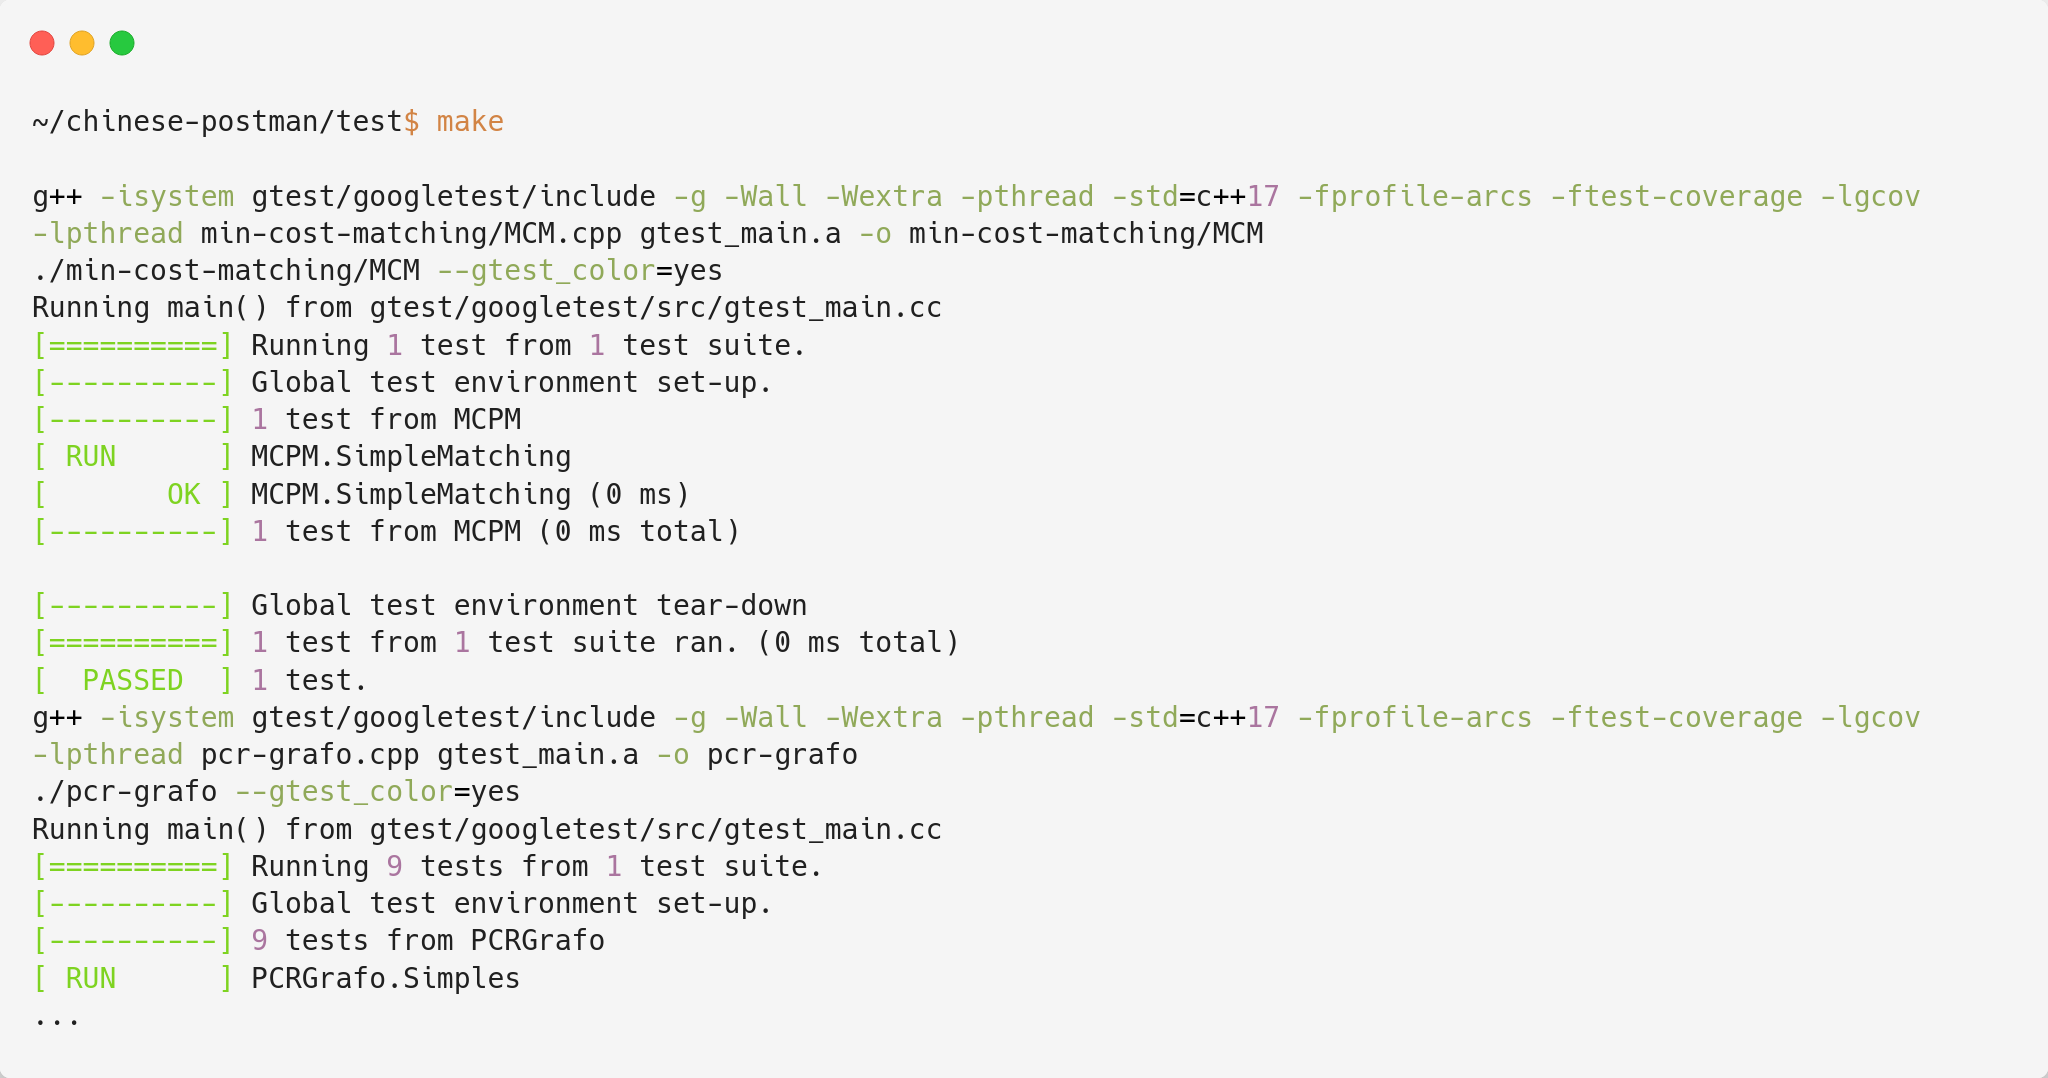
\includegraphics[width=\textwidth]{make-test}
    \caption{Rodando os testes usando o comando \texttt{make}}
    \label{maketest}
\end{figure}

